\documentclass[letterpaper,11pt]{article}
\usepackage[margin=1in,footskip=0.25in]{geometry}
\setlength{\belowcaptionskip}{-11pt}
\usepackage{multirow}
\usepackage{multicol}
\usepackage{indentfirst}
\usepackage{mathtools} 
\usepackage{amssymb}
\usepackage{mathrsfs}
\usepackage{placeins}
\usepackage{tikz}
\usetikzlibrary{scopes}
\usetikzlibrary{shapes,arrows,decorations.markings,plotmarks}
\usepackage[american]{circuitikz}
\usepackage{bondgraphs}
\usepackage{float}
\usepackage{steinmetz}
\usepackage{graphicx}
\usepackage{textcomp}
\usepackage{gensymb}
\usepackage[utf8]{inputenc}
\usepackage{pgfplots}
\usepackage{booktabs}
\usepackage{ulem}
\usepackage{sectsty}
\usepackage{tcolorbox}
\usepackage{hyperref}
\usepackage{siunitx}
\usepackage{xspace}
\usepackage{advdate}
\pgfplotsset{width=10cm,compat=1.9}

\def\doubleunderline#1{\underline{\underline{#1}}}
\newcounter{MyCounter}
\newcommand{\MATLAB}{\textsc{Matlab}\xspace}

%%%% Block Diagram Set-up
\tikzstyle{block} = [draw, fill=white, rectangle, 
    minimum height=3em, minimum width=6em]
\tikzstyle{sum} = [draw, fill=white, circle, node distance=1cm]
\tikzstyle{input} = [coordinate]
\tikzstyle{output} = [coordinate]
\tikzstyle{notation} = [draw,  fill=white, rectangle]
\tikzstyle{pinstyle} = [pin edge={to-,thin,black}]
\tikzstyle{vecArrow} = [thick, decoration={markings,mark=at position
   1 with {\arrow[semithick]{open triangle 60}}},
   double distance=1.4pt, shorten >= 5.5pt,
   preaction = {decorate},
   postaction = {draw,line width=1.4pt, white,shorten >= 4.5pt}]
\tikzstyle{innerWhite} = [semithick, white,line width=1.4pt, shorten >= 4.5pt]

\title{EAE 130B Block Diagram 3}
\author{Yihui Li}
\date{\today}

\begin{document}
\begin{figure}[!htb]
    \centering
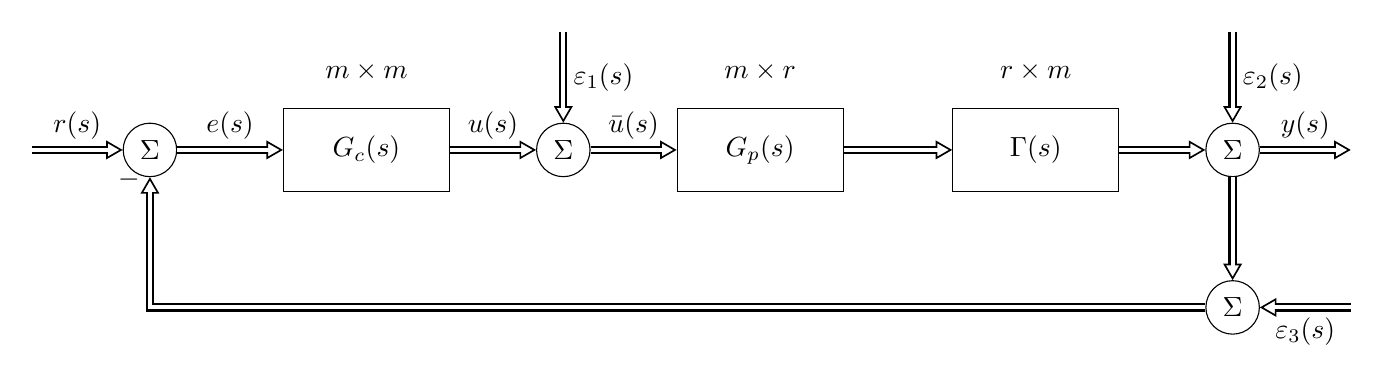
\begin{tikzpicture}[auto, node distance=2cm,>=latex']
% Nodes
	\node [input, name=input] {};
	\node [sum, right of=input, node distance = 1.5 cm] (sum) {$\Sigma$};
	\node [block, right of=sum, node distance = 2.75 cm] (controller) {$G_c(s)$};
	\node [sum, right of=controller, node distance = 2.5 cm] (id) {$\Sigma$};
	\node [block, right of=id, node distance = 2.5 cm] (system) {$G_{p}(s)$};
	\node [block, right of=system, node distance = 3.5 cm] (allocation) {$\Gamma(s)$};
	\node [sum, right of=allocation, node distance = 2.5 cm] (od) {$\Sigma$};  
	\node [input, above of=id, node distance = 1.5 cm] (e1) {};
	\node [input, above of=od, node distance = 1.5 cm] (e2) {};
	\node [output, right of=od, node distance = 1.5 cm] (output) {};
	\node [sum, below of=od, node distance = 2.0 cm] (md) {$\Sigma$};
	\node [input, right of = md, node distance = 1.5 cm] (e3) {};
% Connections
	\draw [vecArrow] (input) -- node {$r(s)$} (sum);
	\draw [vecArrow] (sum) -- node {$e(s)$} (controller);
	\draw [vecArrow] (controller) -- node[name=u] {$u(s)$} (id);
	\draw [vecArrow] (id) -- node[name=f1] {$\bar{u}(s)$} (system);
	\draw [vecArrow] (system) -- node[name=f2] {} (allocation);
	\draw [vecArrow] (allocation) -- node[name=f3] {} (od);
	\draw [vecArrow] (e1) -- node[name=u1] {$\varepsilon_1(s)$} (id);
	\draw [vecArrow] (e2) -- node[name=u2] {$\varepsilon_2(s)$} (od);
	\draw [vecArrow] (e3) -- node[name=u3] {$\varepsilon_3(s)$} (md);
	\draw [vecArrow] (od) -- node [name=y] {$y(s)$}(output);
	\draw [vecArrow] (od) -- (md);
	\draw [vecArrow] (md) -| node[pos=0.99] {$-$} node [near end] {} (sum);
% Notations
	\node [above of = controller, node distance = 1.0 cm] (n1) {$m \times m$};
	\node [above of = system, node distance = 1.0 cm] (n2) {$m \times r$};
	\node [above of = allocation, node distance = 1.0 cm] (n3) {$r \times m$};
\end{tikzpicture}
\caption{Block diagram MIMO}
\label{fig:blockdiagrammimo}
\end{figure}
\end{document}